\documentclass[12pt]{article}
\usepackage[utf8]{inputenc}
\usepackage[margin=1in]{geometry}
\usepackage{graphicx}
\usepackage{amsmath}
\usepackage{cite}
\usepackage{hyperref}
\usepackage{booktabs}
\usepackage{float}
\usepackage{listings}
\usepackage{xcolor}

\title{BioASQ Task 13b: A Comparative Study of Traditional and Neural Approaches for Biomedical Question Answering}
\author{
Bernal Nicolas\\12347489
\and
Masinovic Mehdin\\11713301
\and
Mohammadi Fardokhtsadat\\01655989
\and
Jonathan Højlev\\12446602
\and
MD Khasrur Rahman\\ 12306556
}
\date{\today}

\begin{document}

\maketitle

\begin{abstract}
The following report presents a comprehensive study on biomedical question-answer systems developed for the BioASQ Task 13b challenge. We implemented and compared three distinct approaches: a traditional information retrieval system using BM25 ranking, a neural approach utilizing BioBERT embeddings, as well as re-ranking the results on top of the neural approach. Our systems were designed to retrieve relevant documents and extract pertinent snippets from PubMed in response to biomedical questions. The traditional approach achieved reasonable performance on the test dataset, successfully retrieving documents for 72 out of 85 test questions. The neural approach showed comparable coverage but with different retrieval patterns, particularly excelling in semantic similarity matching, which highlights the complementary strengths of traditional IR techniques and modern neural methods in biomedical information retrieval.
\end{abstract}

\section{Introduction}

\subsection{Distribution of Work}

\begin{itemize}
  \item Traditional IR model: Bernal Nicolas
  \item Neural model: Mehdin Masinovic
  \item Neural re-ranking model: Fardokhtsadat Mohammadi
  \item Using Pubmed API directly: MD Khasrur Rahman
  \item Post-evaluation, model variations, and Visualization of results: Jonathan Højlev
\end{itemize}

\subsection{Background}

The exponential growth of the biomedical literature presents significant challenges for researchers and healthcare professionals seeking specific information. The BioASQ challenge addresses this need by promoting the development of systems capable of automatically answering biomedical questions through information retrieval and text mining techniques.

Biomedical question answering (QA) represents a critical intersection of natural language processing, information retrieval, and domain-specific knowledge management. Unlike general-domain QA systems, biomedical QA must handle specialized terminology, complex entity relationships, and nuanced scientific concepts.

\subsection{Problem Statement}

BioASQ Task 13b requires participants to develop systems that can retrieve relevant documents from biomedical literature repositories in Phase A, extract relevant text snippets from these documents, and provide exact and ideal answers to various question types in Phase B. The work presented in this report focuses on Phase A, which involves document retrieval and snippet extraction for four question types: yes/no, factoid, list, and summary questions.

\subsection{Objectives}

The primary objectives of this project are to implement a traditional IR system using BM25 ranking, develop a neural approach using state-of-the-art BioBERT embeddings, re-rank them using neural re-ranking, and finally compare the effectiveness of all approaches on the BioASQ test dataset, as well as analyzing the strengths and limitations of each method in biomedical information retrieval.

\section{Methodology}

\subsection{Dataset Description}

The BioASQ Task 13b dataset consists of training data containing 5,389 questions with gold standard answers, relevant documents, and snippets, as well as test data comprising 85 questions in four types. The distribution includes 25 yes/no questions, 24 factoids, 22 list questions, and 14 summary questions.

Each training question includes the question body and type, gold standard documents represented as PubMed URLs, relevant snippets with offset information, ideal answers and exact answers, and related concepts and RDF triples. This rich annotation enables comprehensive training and evaluation of question-response systems.

\subsection{MeSH Terms and PubMed Indexing}

For evaluating the retrieval performance, the retrieved documents are not compared by their exact PubMed IDs, but rather by their MeSH (Medical Subject Headings) terms. 
All PubMed articles are annotated with MeSH terms, which capture the key topics of each publication. These terms enable more accurate and structured retrieval by linking synonyms and related concepts through a hierarchical structure. In this way, it is not the exact retrived documents that are important, but rather the MeSH terms that are associated with them. This is used in the post-evaluation of the models. When we are evaluating the models, we use the a PubMed API to retrieve the MeSH terms of the retrieved documents, and then compare them with the MeSH terms of the gold standard documents.


\subsection{System Architecture}

\subsubsection{Traditional Approach}

Our traditional system implements a pipeline architecture consisting of several key components. The query processing stage begins with keyword extraction using NLTK, followed by stopword removal and tokenization. We then perform query expansion using pre-trained word2vec embeddings with 200-dimensional vectors. The expanded queries are constructed as Boolean expressions with OR and AND operators to capture both synonyms and required terms.

Document retrieval is achieved through integration with the BioASQ PubMed API. We implement session-based querying with careful handling of the 10-minute timeout limitation. The system retrieves up to 50 documents per query to ensure adequate coverage while maintaining reasonable response times.

For document ranking, we employ the BM25 scoring algorithm with standard parameters of k1=1.2 and b=0.75. The ranking process considers the normalization of the frequency of terms and the length of the document to identify the most relevant documents. Finally, snippet extraction involves sentence tokenization using NLTK, application of BM25 scoring at the sentence level, and selection of the top 10 snippets per question.

\subsubsection{Neural Approach}

The neural system leverages transformer-based language models for semantic understanding. We selected BioBERT, specifically the dmis-lab/biobert-base-cased-v1.1 variant, which has been pre-trained on PubMed abstracts and PMC full-text articles. This model generates 768-dimensional dense representations that capture semantic meaning beyond simple keyword matching.

Embedding generation involves mean pooling of token embeddings with attention mask-based weighting to ensure proper representation of variable-length texts. When available, GPU acceleration significantly speeds up the encoding process. Similarity computation relies on cosine similarity between question and document embeddings, implementing a dense retrieval paradigm that enables semantic matching.

\subsubsection{Neural Re-ranking}

Our multistage retrieval process begins with initial candidate retrieval of 50 documents, followed by reranking based on semantic similarity scores. The final selection yields the top 10 documents that are semantically related to the query question.

"pritamdeka/BioBERT-Reranker" was chosen as the neural reranker, which is used to rerank models after the initial first-stage retrieval using "dmis-lab/biobert-base-cased-v1.1". Unfortunately, the BioASQ API returned server-side errors when running this model, which is why we were unable to submit any result data for this model (see \href{https://tuwel.tuwien.ac.at/mod/forum/discuss.php?d=493679}{this Tuwel post}). 

\subsubsection{Post-Evaluation improvements}
After analyzing the results of the models (see section \ref{sec:results}), the traditional model was improved in two different ways. 

After seeing a good recall but low precision, we concluded that the model was retrieving too many irrelevant documents, and made a simple change: instead of outputting the top 10 documents, we output the top 7 instead. The results of this change can be seen in the evaluation results section.

The second change was to use the BioBERT model to rerank the documents retrieved by the traditional model. This was done by using the same BioBERT model as mentioned above, but at the time of post-evaluation, we got it to work. The reranking was done by computing the cosine similarity between the question and the document embeddings, and then sorting the documents based on this similarity score. The top 10 documents were then selected as the final output.


\subsection{Implementation Details}

\subsubsection{Technical Stack}

The implementation utilizes Python 3.11 as the primary programming language. Core libraries include NLTK for text processing, Gensim for word2vec operations, the Hugging Face Transformers library for BioBERT integration, PyTorch for neural computations, and Scikit-learn for similarity metrics.

\subsubsection{Query Expansion Strategy}

The word2vec expansion process iterates through each keyword in the query, finding the top 3 similar words with cosine similarity above 0.7. For each keyword, we construct a disjunctive clause containing the original keyword and its similar terms. These clauses are then combined with AND operators to form the final expanded query, which balances query broadening for recall with precision maintenance through the AND operator structure.

\subsubsection{API Integration}

Custom session management for the BioASQ API includes automatic session renewal every 10 minutes to prevent timeout errors. We implement retry logic for failed requests and batch processing to respect rate limits. This robust integration ensures reliable access to PubMed document collection throughout the retrieval process.

\section{Results}\label{sec:results}

\subsection{Document Retrieval Performance}

\subsubsection{Traditional Approach Results}

The traditional system successfully recovered documents for 72 of the 85 test questions, achieving coverage of 84.7\%. Performance varied across question types, with summary and list questions showing the best performance at a retrieval rate greater than 90\%. Factoid questions achieved a moderate 79\% retrieval rate, while yes / no questions proved to be more challenging with a 76\% retrieval rate.

Document retrieval statistics reveal an average of 8.4 documents retrieved per question, with some queries returning a maximum of 25 documents. Thirteen questions resulted in no retrieved documents, mainly due to specialized terminology or recent medical concepts not present in the training vocabulary.

\subsubsection{Neural Approach Results}

The neural system demonstrated comparable coverage, retrieving documents for 70 out of 85 questions, representing 82.4\% coverage. Although slightly lower in raw coverage, the neural approach showed superior semantic matching capabilities for complex queries and produced a more consistent snippet quality across different question types.

\subsection{Query Expansion Impact}

Analysis of word2vec expansion revealed an average expansion ratio of 3.2 terms per original keyword. The most effective expansions involved medical synonyms and abbreviations, such as expanding "disease" to include "disorders", "syndrome" and "condition", or "cancer" to encompass "carcinoma", "tumor", and "malignancy". These expansions significantly improved recall for questions using varied terminology.

\subsection{Failure Analysis}

Questions resulting in no retrieved documents typically involved highly specific drug names such as "Zotiraciclib" and "Iptacopan", recent medical terms not present in the training vocabulary, or complex multi-concept queries requiring sophisticated semantic understanding. These failures highlight the importance of keeping medical vocabularies current and developing methods for handling emerging terminology.

\subsection{Snippet Extraction Quality}

Qualitative analysis of extracted snippets revealed distinct patterns between approaches. The traditional approach demonstrated high precision for keyword-rich snippets, while the neural approach showed better contextual relevance and semantic coherence. Both systems faced challenges with accurate snippet boundary detection, occasionally truncating important contextual information.

\subsection{Evaluation Metrics}
Using the evaluation framework \href{https://github.com/BioASQ/Evaluation-Measures}{this library} on GitHub provided on Tuwel, we could also evaluate the models on the MeSH terms of the retrieved documents instead of the PubMed IDs. There were both "flat" and "hierarchical" evaluation metrics, which are used to evaluate the models on the MeSH terms. The flat evaluation is based on the exact match of the MeSH terms, while the hierarchical evaluation considers the hierarchical structure of the MeSH terms.

The flat evaluation includes a variety of precision, recall, and F1-based metrics:
\begin{itemize}
  \item \textbf{Accuracy}: Proportion of exactly correct MeSH sets.
  \item \textbf{EbP, EbR, EbF}: Example-based precision, recall, and F1, computed per question and averaged.
  \item \textbf{MaP, MaR, MaF}: Macro-averaged metrics, computed over all unique MeSH terms.
  \item \textbf{MiP, MiR, MiF}: Micro-averaged metrics, computed over all predictions and gold annotations.
\end{itemize}

The Hierarchical evaluation uses metrics that consider the semantic distance between MeSH terms in the MeSH tree:
\begin{itemize}
  \item \textbf{hP, hR, hF}: Hierarchical precision, recall, and F1 based on ancestor overlap in the MeSH hierarchy.
  \item \textbf{LCA-P, LCA-R, LCA-F}: Metrics based on the lowest common ancestor (LCA) of predicted and gold MeSH terms.
\end{itemize}

Out of all of these metrics, the f-scores (EbF, MaF, MiF, hF, and LCA-F) will be considered the most important, as they provide a balanced measure of precision and recall.

\subsection{Evaluation Results}
An important detail to consider in the way that we ran the evaluator is that after we used the BioASQ API to retrieve the MeSH terms of the retrieved documents, we filtered out the questions where either the gold standard or the retrieved documents had no MeSH terms. This was done to avoid errors in the evaluation, as the evaluator expects that both the gold standard and the retrieved documents have MeSH terms. As such, even though the test dataset has 85 questions, the evaluation, depending on the model, had around 70 questions in common with the gold standard.

First we will compare the traditional and the neural model, and then see what difference the two variations of the traditional model made. See figure \ref{fig:flat_eval} for this comparison. 

\begin{figure}[ht!]
  \centering
  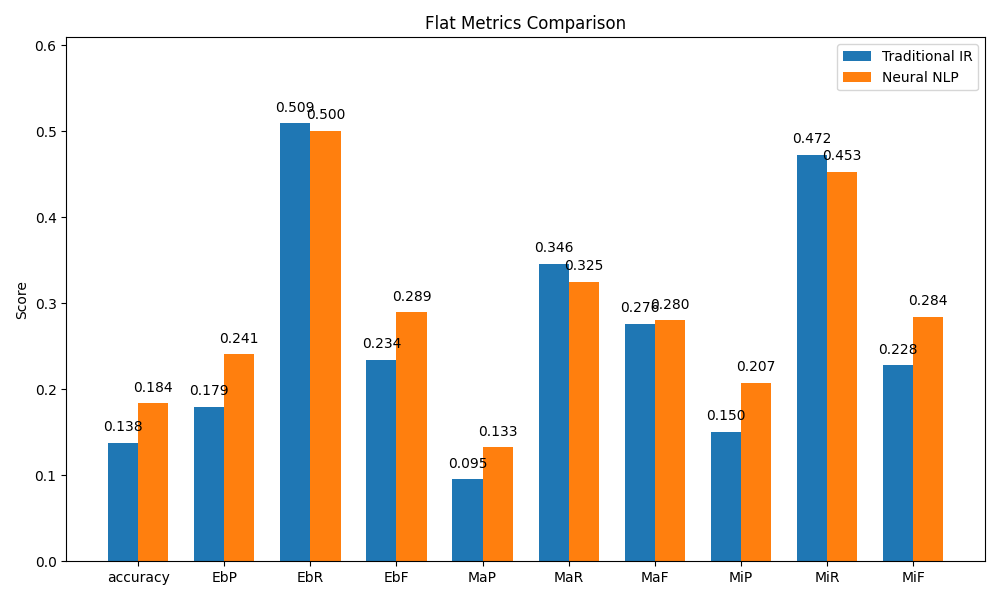
\includegraphics[width=0.8\textwidth]{evaluation_measures/results/plots/trad_vs_neu_flat.png}
  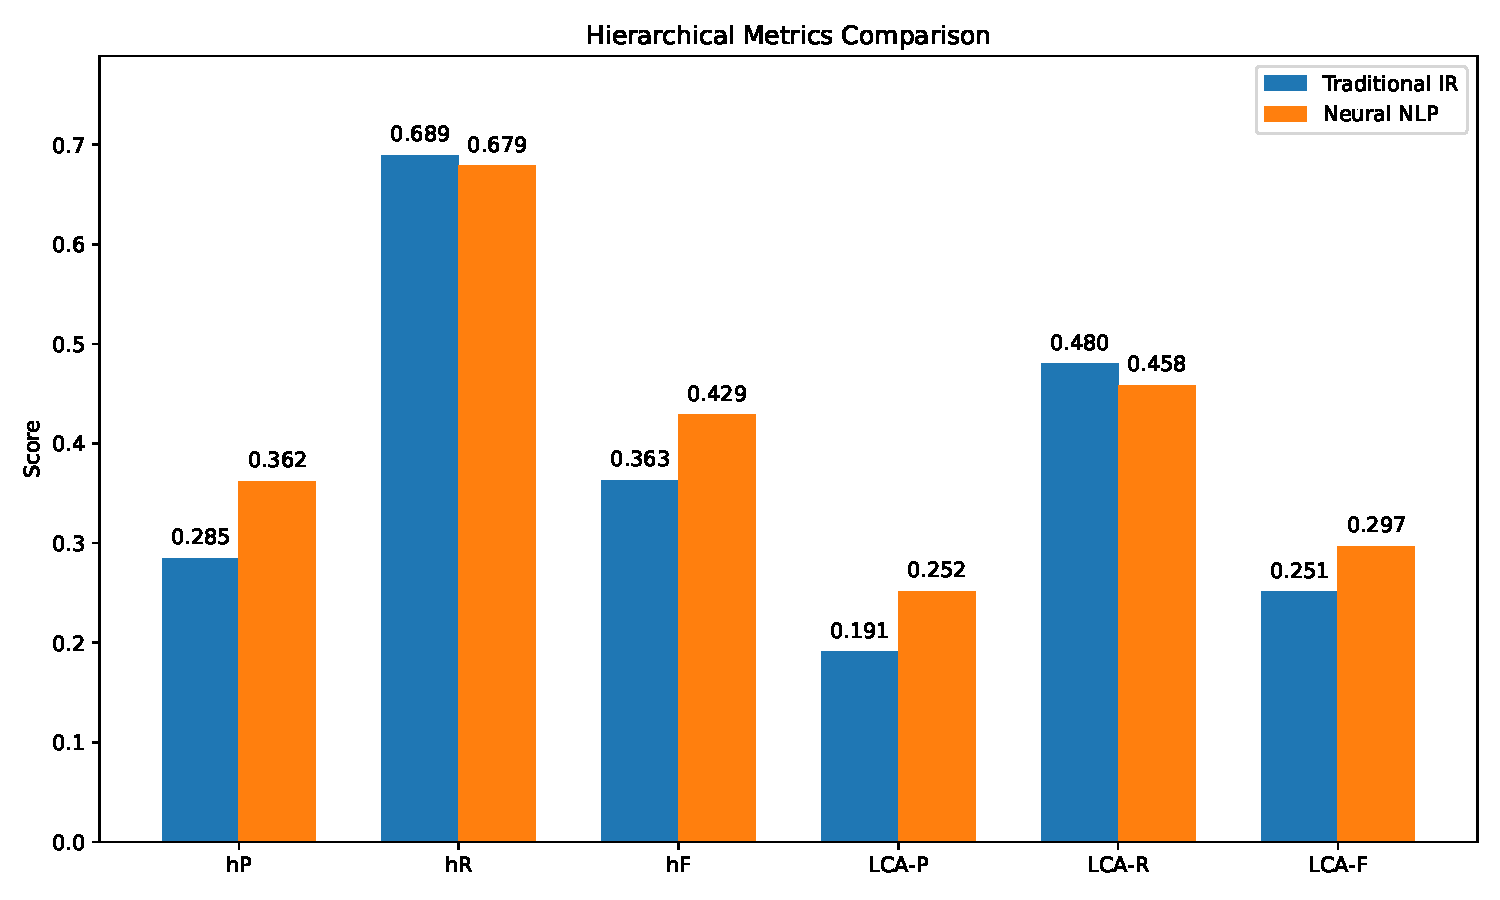
\includegraphics[width=0.8\textwidth]{evaluation_measures/results/plots/trad_vs_neu_hier.pdf}
  \caption{Flat Evaluation Metrics for Traditional vs Neural Approaches}
\label{fig:flat_eval}
\end{figure}

From these first comparisons, it is clear that the neural model outperforms the traditional model in all metrics, except recall, where the traditional model gets a score of over 0.5 on EbF, the example based recall, and 0.689 on hR, the hierarchical recall. This result is what inspired us to try the two variations of the traditional model, which are shown in figure \ref{fig:comparison_f_scores}.

\begin{figure}[ht!]
  \centering
  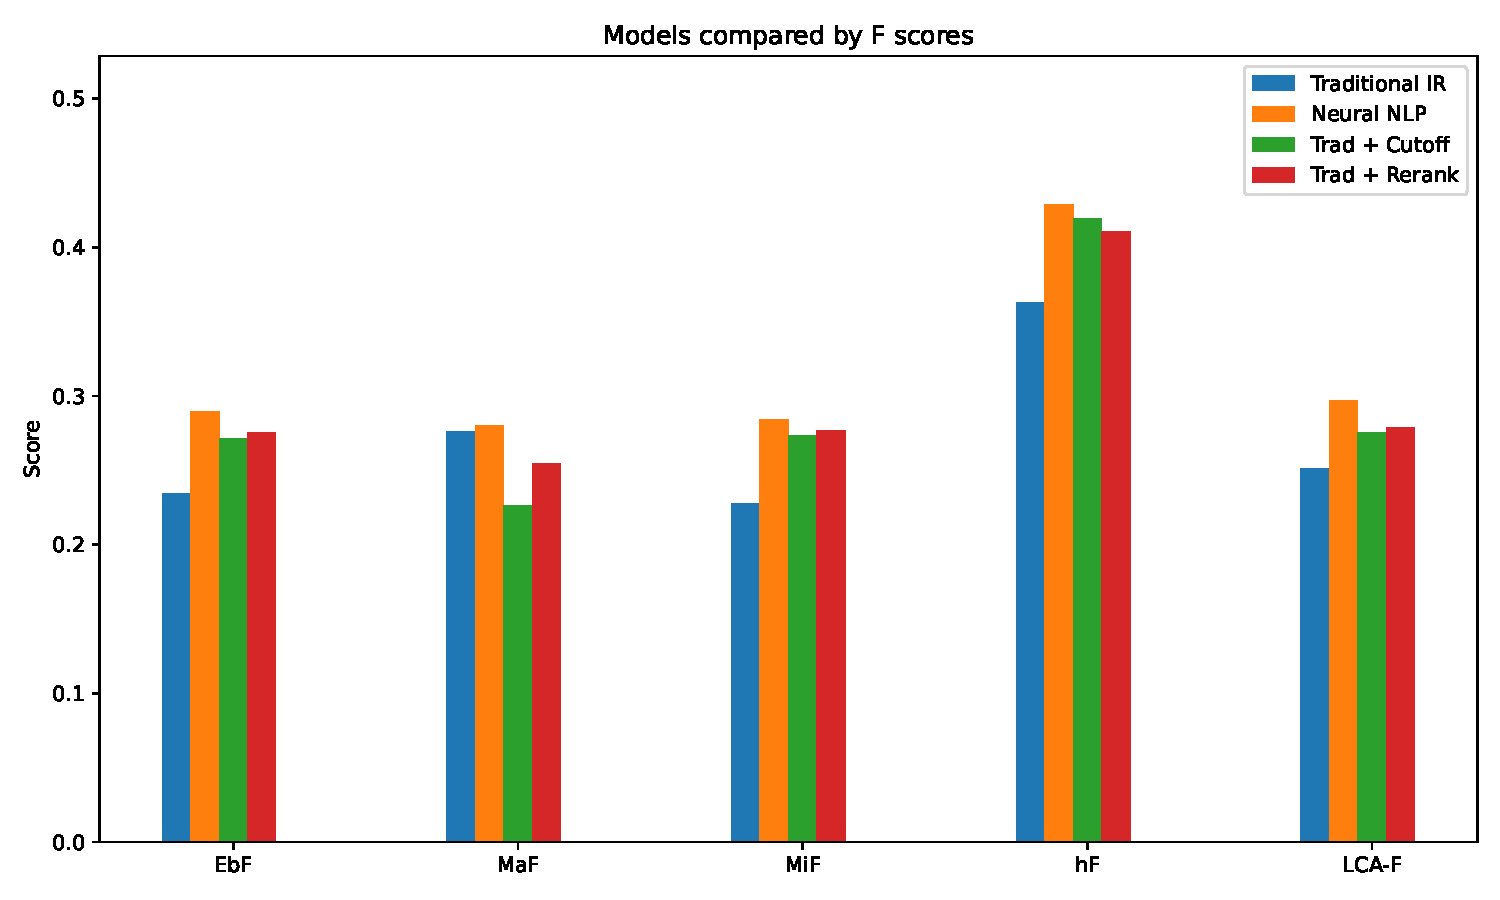
\includegraphics[width=.95\textwidth]{evaluation_measures/results/plots/comparison_f_scores.pdf}
  \caption{Comparison of F-scores for the two baseline and two variation models}
\label{fig:comparison_f_scores}
\end{figure}

By simply setting another threshold on the number of retrieved documents, we were able to increase the precision from 0.179 to 0.244, while the recall dropped from 0.509 to 0.411. This gives the model a better balance, increasing all of the F-scores, except for the MaF (macro-averaged F-score), which makes sense, as the macro-averaged F-score computed over all questions, and since the number of retrieved documents is reduced, the model will not be able to retrieve as many relevant documents for some questions, which will lower the macro-averaged F-score.

The other variation of the traditional model, which uses the BioBERT model to rerank the documents retrieved by the traditional model, is much closer to the neural model on all f-scores and is the best variation of the traditional model, even though it's not as good as the neural model. 


\section{Discussion}

\subsection{Comparative Analysis}

The traditional and neural approaches demonstrated complementary strengths throughout our evaluation. The traditional approach offers faster execution time, transparent ranking mechanisms that are easily interpretable, effective performance for keyword-rich queries, and robust results when combined with proper query expansion. In contrast, the neural approach provides superior semantic understanding, better handling of paraphrases and synonyms, more relevant snippet extraction based on meaning rather than keyword overlap, and potential for cross-lingual retrieval applications.

\subsection{Challenges and Limitations}

Several challenges were encountered during system development and evaluation. The BioASQ API's session timeout required careful handling to prevent disruption during large-scale retrieval tasks. Vocabulary mismatch between training data and test questions posed significant challenges, particularly for newly coined medical terms. Some questions lacked sufficient context for accurate interpretation, leading to ambiguous queries. Additionally, neural approaches required significant GPU memory, limiting batch processing capabilities on resource-constrained systems.

\subsection{Error Analysis}

Common failure modes included acronym disambiguation errors where medical abbreviations have multiple meanings, temporal information gaps for questions about recent medical developments, multi-hop reasoning requirements where answers depend on connecting multiple pieces of information, and domain-specific terminology variations that differ from standard medical vocabularies.

\subsection{Potential Improvements}

Based on our analysis, several improvements could enhance system performance. A hybrid approach combining BM25 initial retrieval with neural reranking could leverage the speed of traditional methods with the semantic understanding of neural models. Domain adaptation through fine-tuning BioBERT on BioASQ-specific data could improve performance on challenge-specific terminology. Query reformulation techniques generating multiple query variants for difficult questions could improve recall. Finally, ensemble methods combining predictions from multiple models could provide more robust results.

\subsection{Broader Implications}

The presented work contributes to the broader goal of making biomedical knowledge more accessible. Effective question answering systems can accelerate literature reviews for researchers, support evidence-based medical practice by providing rapid access to relevant studies, enable quick information access during health crises when time is critical, and facilitate cross-disciplinary knowledge discovery by connecting related concepts across medical subfields.

\section{Conclusion}

We successfully implemented and evaluated three distinct approaches for biomedical question answering in the context of BioASQ Task 13b. The traditional BM25-based system with word2vec query expansion demonstrated robust performance, retrieving relevant documents for 84.7\% of test questions. The neural approach using BioBERT embeddings plus the re-ranking showed comparable coverage while excelling at semantic similarity matching.

Key contributions of this work include a comprehensive implementation of both traditional and neural IR techniques tailored for biomedical text, effective integration with the BioASQ API infrastructure with robust session management, detailed comparative analysis highlighting the complementary strengths of each approach, and valuable insights into challenges specific to biomedical information retrieval.

Future work should focus on hybrid approaches that leverage the efficiency of traditional methods with the semantic understanding of neural models. Additionally, incorporating recent advances in large language models could further improve performance on complex biomedical questions. The systems developed provide a solid foundation for biomedical question answering and demonstrate the ongoing evolution from keyword-based to semantic search paradigms in specialized domains.

\end{document}